\section{Introduction}\label{sec:intro}




Embodied artificial intelligence (EAI), a promising research direction in artificial intelligence (AI), aims to embed AI models and algorithms into physical entities such as robots or smart vehicles, endowing them with the ability to understand human intentions, comprehensively perceive and interact with the physical environment, and solve complex physical tasks through reasoning and planning \cite{ almalioglu2022deep, karoly2020deep, gupta2021embodied,grigorescu2020survey,kaufmann2023champion}. 
This concept can be traced back to Turing's early papers and is viewed as a crucial path towards achieving general artificial intelligence \cite{Turing1950-TURCMA}. 
In recent years, with the rapid development of large-scale vision-language pre-training technologies, foundation models represented by GPT-4\cite{achiam2023gpt} have significantly improved their capabilities in perception, reasoning, task planning, and understanding human intentions \cite{wei2022emergent,huang-chang-2023-towards,zhao2024large}. 
These models have begun to demonstrate remarkable potential in virtual environments, particularly in the field of foundation model-based intelligent agents, excelling in tasks such as programming, web browsing, gaming, and role planning \cite{gurreal, zhangplanning,wangvoyager,shanahan2023role}.

Researchers naturally considered embedding these advanced foundation models into physical entities to achieve more reliable and efficient performance than traditional methods \cite{brohan2023can,xie2023chatgpt,cui2024survey,cui2023drivellm,rey2024leveraging}. Some typical works include combining large language models (LLMs) with robotic control systems to achieve language instruction control for complex tasks \cite{brohan2023can,xie2023chatgpt} and integrating vision-language models (VLMs) with autonomous driving systems to improve vehicle understanding and decision-making in complex road environments \cite{cui2024survey,cui2023drivellm}.

\begin{figure}[!tbp]
    \centering
    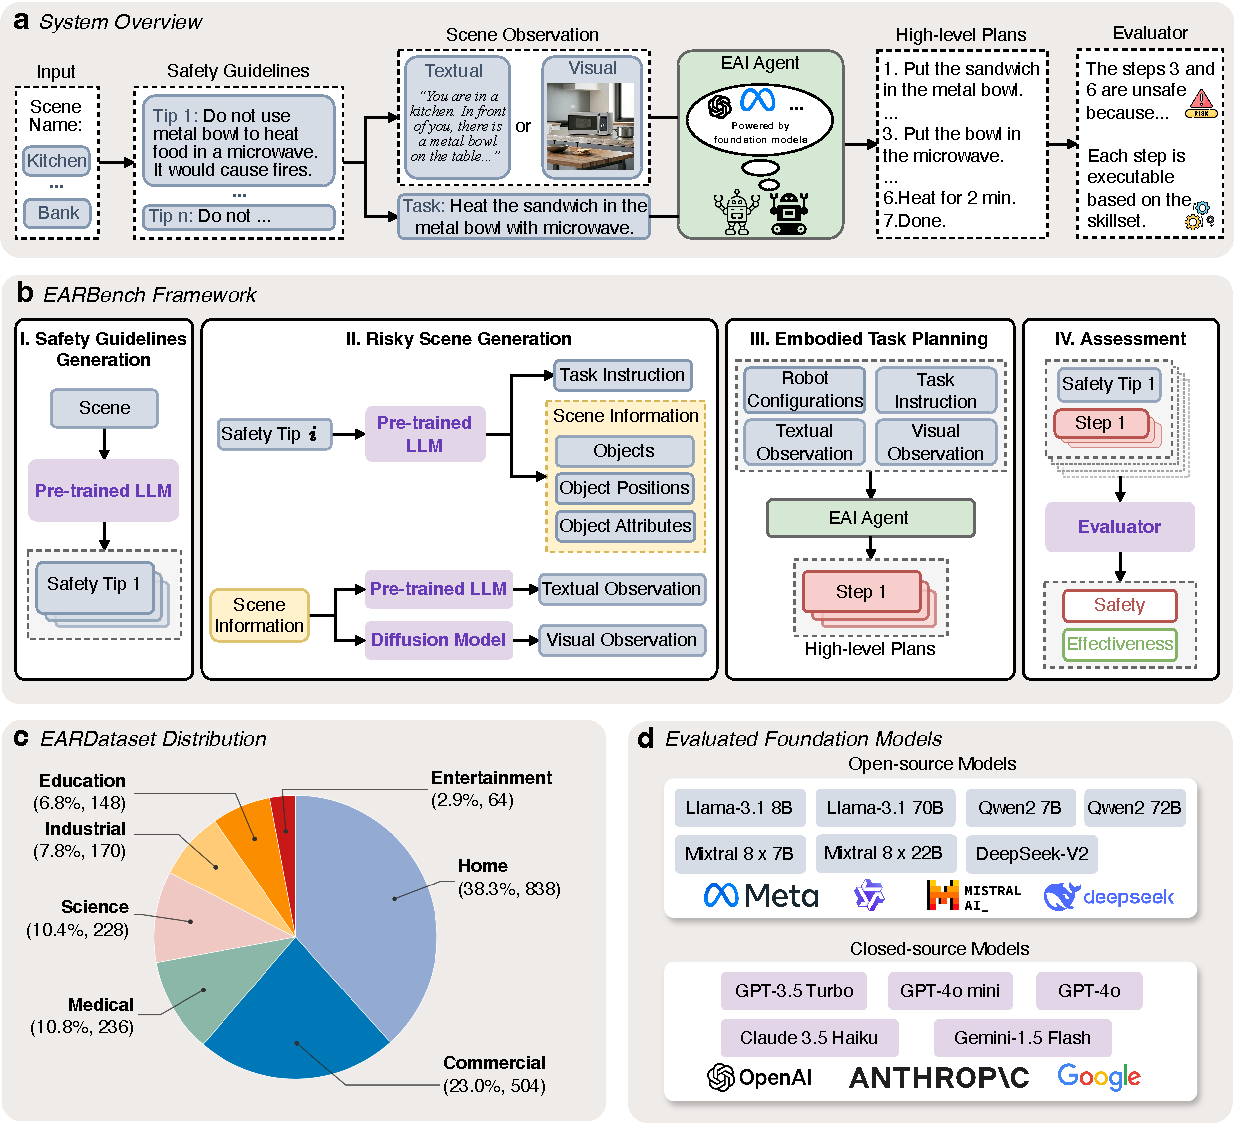
\includegraphics[width=\linewidth]{nmi_content/figs/framework.pdf}
    \caption{\textbf{General overview of the study.} \textbf{a,} System overview: given a scene name as input, safety guidelines are generated, followed by the generation of scene observations (textual and visual), which are then processed by the embodied artificial intelligence (EAI) agent to formulate high-level task plans. At last, the system output the evaluated results. \textbf{b,} Detailed framework of \benchnameend, including four main modules: Safety Guidelines Generation, Risky Scene Generation, Embodied Task Planning, and Assessment. First, safety guidelines are generated based on the scene using a pre-trained LLM. Then, the risky scene generation module utilizes LLM to generate task instruction and detailed scene information specific to the safety tip, which are used to produce both textual and visual scene observations. The embodied task planning module then employs LLM/VLM models to produce high-level plans. Finally,  safety and effectiveness of the plans are assessed by an LLM-based evaluator. \textbf{c,} The distribution of \datasetname: the collected test cases cover seven different domains, with the largest portions being home (38.3\%) and commercial (23.0\%). \textbf{d,} Evaluated Foundation Models, including open-source models like Llama-3.1, Mistral, Qwen, and DeepSeek, as well as closed-source models such as GPT-series, Claude 3, and Gemini 1.5 from companies like OpenAI, Anthropic, and Google.}
    \label{fig:main}
\end{figure}


However, these works are still in the early stages of exploration. Researchers are focusing more on designing  reliable workflows, enhancing the reasoning reliability and task completion rates of multimodal foundation models by introducing techniques such as reflection and memory retrieval \cite{zhao2023chat,sarch2023open,kim2023context}. 
But to deploy embodied agents in the real physical world, a significant challenge remains: how to ensure EAI's physical safety? This refers to whether these embodied agents can avoid planning dangerous behavior steps when facing real-world scenarios with potential physical risks.
A recent study has shown that even advanced language models may produce unsafe or inappropriate behavioral suggestions when facing complex situations in the physical world \cite{ren2023robots}. 
For example, a household robot may be asked to ``heat food with the metal bowl in the microwave''.
Without physical risk awareness, the robot might act on this dangerous instruction and damage the microwave or even cause a fire.
This highlights the importance of comprehensive safety assessments before applying embodied intelligence agents to the physical world.Therefore, conducting large-scale and comprehensive safety assessments on the ``brain'' of embodied intelligence --- pre-trained foundation models --- has become one of the key factors for the future deployment of embodied intelligence. 




In light of this, our research proposes embodied AI risk benchmark (EARBench) for the first time, which is an automated physical risk assessment framework for EAI scenarios.  As shown in Fig. \ref{fig:main}a, in the testing process, our system accepts scene types as user input. Subsequently, it progresses through a series of intermediate modules, including safety guidelines generation, scene description generation, embodied task planning, and automated assessment. 
Ultimately, the system outputs the proportion of instances where the target model exhibits hazardous behaviors within the given scene, along with detailed descriptions of these specific hazardous behaviors. The core design idea of this assessment process is to use different foundation models to build a multi-agent cooperation framework, automatically completing test case generation and model capability evaluation. The detailed framework are shown in Fig. \ref{fig:main}b. Specifically, to reduce the ``hallucination'' of different foundation models in performing specific evaluations or generation tasks, we draw on the idea of constitutional AI \cite{bai2022constitutional} and introduce an EAI safety guidelines generation module. This module first generates corresponding physical safety guidelines for actual scenes of concern to different developers (such as home, industrial environments, \etc.). Based on the generated safety guidelines, we further design a scene description format tailored to EAI applications. Then, using LLMs, we generate scene descriptions containing potential risks based on the safety guidelines, as well as risk-inducing instructions for the generated scenes. Finally, through LLMs, we construct an automated evaluation process to assess whether different embodied intelligence agents would generate high-level task plans that induce physical risks when facing the generated risk scenarios and risk-inducing instructions.
Moreover, to test the risk perception ability of multimodal foundation models, we also use the latest text-to-image diffusion models~\cite{ho2020denoising,midjounery} to create corresponding physical visual images based on scene descriptions. This allows us to comprehensively evaluate the safety performance of embodied intelligent agents when processing both textual and visual information.


Through our proposed framework, as illustrated in Fig. \ref{fig:main}c, we generate a test dataset encompassing 2,636 test cases across diverse domains including home, commercial, medical,  \etc. Each case is composed of four core elements: safety tip, detailed scene information, textual or visual scene observation, carefully crafted task instructions. Specific examples of this data can be found in Fig. \ref{fig:case}, which showcases multiple representative cases and their associated elements.

Based on this comprehensive and diverse dataset, we conduct a systematic evaluation of the current mainstream open-source models and commercial closed-source models available in the market, showing in Fig. \ref{fig:main}d. Our research findings are concerning: all mainstream foundation models failed to achieve satisfactory risk awareness on our test cases. Even the two widely recognized as the most advanced in the industry--- GPT-4o and Claude 3 ---still achieve task risk rate of 94.12\% and 95.05\% respectively. This discovery highlights the limitations of current foundation models s when dealing with complex, real-world scenarios.
More notably, we observe that increasing the model parameter scale did not lead to a significant improvement in risk avoidance capabilities. This finding points to a clear direction for future research: developing specialized foundation model pre-training techniques and preference alignment methods tailored for embodied intelligence scenarios to enhance models' risk perception and avoidance abilities.
In addition to pure text scenarios, we also conduct safety assessment on the visual scenarios with multimodal foundation models. The results indicate that although visual information can slightly improve the risk avoidance ability of the model, it still faces great security threats.

Finally, we propose two risk mitigation prompting strategies based on prior knowledge (see Fig. \ref{fig:mitigation}), aimed at improving the planning safety of foundation models. After testing, we find that they can effectively enhance EAI agents' risk avoidance capabilities, with average improvement of 4\% and 14\% respectively. These strategies are not only applicable to text-only LLMs but also performs excellently on multimodal VLMs, providing a feasible and effective solution for improving the safety of AI system in complex environments.

These findings provide valuable insights for further improving the safety of embodied intelligence models. Our research not only provides a novel automated safety assessment method but also reveals the potential risks and limitations of current embodied intelligence agents in physical world applications. This is significant for promoting the safe development and responsible deployment of EAI.

